\documentclass{article} % For LaTeX2e
\usepackage{nips13submit_e,times}
\usepackage{graphicx}
\usepackage{subfig}
\usepackage{hyperref}
\usepackage{amsmath}
\usepackage{algorithm}
\usepackage{multirow}
\usepackage[noend]{algpseudocode}
\usepackage{multirow,multicol, makecell, booktabs}
\usepackage{url}
%\documentstyle[nips13submit_09,times,art10]{article} % For LaTeX 2.09

\makeatletter
\def\BState{\State\hskip-\ALG@thistlm}
\makeatother

\title{Word2Bits - Quantized Word Vectors}


\author{
Maximilian Lam\\
\texttt{maxlam@stanford.edu} \\
}

\newcommand{\fix}{\marginpar{FIX}}
\newcommand{\new}{\marginpar{NEW}}

\nipsfinalcopy % Uncomment for camera-ready version

\begin{document}


\maketitle

\begin{abstract}
Word vectors require significant amounts of memory and storage, posing
issues to resource limited devices like mobile phones and GPUs. We
show that high quality quantized word vectors using 1-2 bits per
parameter can be learned by training Word2Vec with a quantization
function. We furthermore show that training with the quantization
function acts as a regularizer. We train word vectors on full english
Wikipedia (2017) and evaluate them on standard word similarity and
analogy tasks and on question answering (SQuAD). Our quantized word
vectors not only take 8-16x less space than full precision (32 bit)
word vectors but also outperform them on word similarity tasks and
question answering.
\end{abstract}

\section{Introduction}
Word vectors are extensively used in deep learning models for natural
language processing. Each word vector is typically represented as a
300-500 dimensional vector, with each parameter being 32 bits. As
there are millions of words, word vectors may take up to 3-6 GB of
memory/storage -- a massive amount relative to other portions of a
deep learning model[1]. These requirements pose issues to
memory/storage limited devices like mobile phones and GPUs.

Furthermore, word vectors are often re-trained on application specific
data for better performance in application specific domains[1]. This
motivates directly learning high quality compact word representations
rather than adding an extra layer of compression on top of pretrained
word vectors which may be computational expensive and degrade
accuracy.

Recent trends indicate that deep learning models can reach a high
accuracy even while training in the presence of significant noise and
perturbation[1]. It has furthermore been shown that high quality
quantized deep learning models for image classification can be learned
at the expense of more training epochs[1]. Inspired by these trends we
ask: can we learn high quality word vectors such that each parameter
is only one of two values, or one of four values (quantizing to 1 and
2 bits respectively)?

To that end we propose learning quantized word vectors by introducing
a quantization function into the Word2Vec loss formulation -- we call
our simple change Word2Bits. While introducing a quantization function
into a loss function is not new, to the best of our knowledge it is
the first time it has been applied to learning compact word representations.

In this report we show that
\begin{enumerate}
\item[$\bullet$]

  It is possible to train high quality quantized word vectors which
  take 8x-16x less storage/memory than full precision word
  vectors. Experiments on both intrinsic and extrinsic tasks show that
  our learned word vectors perform comparably or even better on many tasks.

\item[$\bullet$]

  Standard Word2Vec may be prone to overfitting; the quantization
  function acts as a regularizer against it.

\end{enumerate}

\section{Related Work}
Word vectors are continuous representations of words and are used by
most deep learning NLP models. Word2Vec, introduced by Mikolov's
groundbreaking papers[1], is an unsupervised neural network algorithm for
learning word vectors from textual data. Since then, other
groundbreaking algorithms (Glove, FastText) [1] have been proposed to
learn word vectors using other properties of textual data. As of 2018
the most widely used word vectors are Glove, Word2Vec and
FastText. This work focuses on how to learn memory/storage efficient
word vectors through quantized training -- specifically our approach
extends Word2Vec to output high quality quantized word vectors.

Learning compact word vectors is related to learning compressed neural
networks. Finding compact representations of neural
networks date back to the 90's and include techniques like network
pruning[1], knowledge distillation[1], deep compression[1] and
quantization[1]. More recently, algorithmic and hardware advances have
allowed training deep models using low precision floating-point and
arithmetic operations[1] -- this is also referred to as
quantization. To distinguish between quantized training with low
precision arithmetic/floats from quantized training with full
precision arithmetic/floats but constrained values we term the first
physical quantization and the latter virtual quantization.

Our technical approach follows that of neural network quantization for
image classification[1], which does virtual quantization by
introducing a sign function (a 1 bit quantization function) into the
training loss function. The actual technique of backpropagating through a
discrete function (the quantization function) has been thoroughly
explored by Hinton[1] and Bengio[1].

Application wise, various techniques exist to compress word
embeddings[1]. These approaches involve taking pre-trained word
vectors and compressing them using dimensionality reduction[1],
pruning[1], or more complicated approaches like deep compositional
coding[1]. Such techniques add an extra layer of computation to
compress pre-trained embeddings and may degrade word vector
performance[1].

To the best of our knowledge, current traditional methods of obtaining
compact word vectors involve adding an extra layer of computation to
compress pretrained word vectors[1] (as described previously). This
may incur computational costs which may be expensive in context of
retraining word vectors for application specific purposes and may
degrade word vector performance[1]. Our proposed approach of directly
learning quantized word vectors from textual data may amend these
issues and is an alternative method of obtaining compact high quality
word vectors. Note that these traditional compression methods may
still be applied on the learned quantized word vectors.

\section{Word2Bits - Quantized Word Embeddings}
\subsection{Background}
Our approach utilizes the Word2Vec formulation of learning word vectors. There
are two Word2Vec algorithms: Skip Gram Negative Sampling (SGNS) and
Continuous Bag of Words (CBOW)[1] -- our virtual quantization
technique utilizes CBOW with negative sampling. The CBOW negative
sampling loss function minimizes

$$
J(u_o, \hat{v}_c) = -log(\sigma(u_o^T\hat{v}_c)) - \sum_{i=1}^{k} log(\sigma(-u_i^T\hat{v}_c))
$$

where

$$
u_o = \mbox{ vector of center word with corpus position } o
$$
$$
\hat{v}_c = \frac{1}{2w-1}\sum_{-w+o \leq i \leq w+o,i \neq o} v_i \mbox{  where } v_i \mbox{ is vector for context word, } w \mbox{ is window size, a hyperparameter}
$$
$$
k = \mbox{ number of negative samples, a hyperparameter}
$$

Intuitively, minimizing this loss function optimizes vectors of
words that occur in similar contexts to be ``closer'' to each other,
and pushes vectors whose contexts are different ``away''. Specifically CBOW with negative sampling tries to predict the
center word from context words.

Technically, to optimize this loss function, for each window of words:

\begin{enumerate}

\item[$\bullet$] Identify the center word's vector $u_o$ within the window
\item[$\bullet$] Compute the average of the context words $\hat{v}_c = \frac{1}{2w-1} \sum_{-w+o \leq i \leq w+o, i \neq o} v_i$ given window size $w$
\item[$\bullet$] Draw $k$ negative samples $u_1, u_2, .., u_k$ according to a sampling distribution [1].
\item[$\bullet$] Compute loss $J(u_o, \hat{v}_c) = -log(\sigma(u_o^T\hat{v}_c)) - \sum_{i=1}^{k} log(\sigma(-u_i^T\hat{v}_c))$
\item[$\bullet$] Update center word vector $u_o$ with gradient $\frac{\partial J(u_o, \hat{v}_c)}{\partial u_o}$
\item[$\bullet$] Update negative word vector $u_i$ with gradient $\frac{\partial J(u_o, \hat{v}_c)}{\partial u_i}$
\item[$\bullet$] Update context word vector $v_i$ with gradient $\frac{\partial J(u_o, \hat{v}_c)}{\partial v_i}$
\end{enumerate}

Center vectors $u_i$ and context vectors $v_j$ are stored full
precision. The final word vectors are the sums of the context and
center vectors $u_i + v_i$ for each corresponding word. The resulting
vectors are full precision.

\subsection{Word2Bits Approach}
To learn quantized word vectors we introduce virtual quantization into the CBOW loss function:
$$
J_{quantized}(u^{(q)}_o, \hat{v}^{(q)}_c) = -log(\sigma((u^{(q)}_{o})^{T} \hat{v}^{(q)}_c)) - \sum_{i=1}^{k} log(\sigma((-u^{(q)}_i)^T\hat{v}^{(q)}_c))
$$

where

$$
u^{(q)}_o = Q_{bitlevel}(u_o)
$$

$$
\hat{v}^{(q)}_c = \sum_{-w+o \leq i \leq w+o,i \neq o} Q_{bitlevel}(v_i)
$$

$$
Q_{bitlevel}(x) = \mbox{ quantization function to quantize to } bitlevel \mbox{ bits}
$$

The following quantization functions were used (chosen based on what worked best)

\[
Q_1(x) =
\begin{cases}
  \frac{1}{3} & x \geq 0\\
  -\frac{1}{3} & x < 0
\end{cases}
\]


\[
Q_2(x) =
\begin{cases}
  \frac{3}{4} & x > \frac{1}{2}\\
  \frac{1}{4} & 0 \leq x \leq \frac{1}{2}\\
  -\frac{1}{4} & -\frac{1}{2} \leq x < 0\\
  -\frac{3}{4} & x < -\frac{1}{2}
\end{cases}
\]

Since $Q_{bitlevel}$ is a discrete function, its derivative is
undefined at some points and 0 at others. To solve this we simply set
the derivative of $Q_{bitlevel}$ to be the identity function:

$$
\frac{\partial Q_{bitlevel}(x)}{\partial x} = I
$$

This is also known as Hinton's straight-through estimator[1].

The final gradient updates reduce to Word2Vec updates. They are:
$$
\mbox{For center word } u_o \textbf{: } \frac{\partial J_{quantized} (u^{(q)}_o, \hat{v}^{(q)}_c)}{\partial u_o} = \frac{\partial J_{quantized} (u^{(q)}_o, \hat{v}^{(q)}_c)}{\partial u^{(q)}_o}
$$
$$
\mbox{For negative word } u_i \textbf{: } \frac{\partial J_{quantized} (u^{(q)}_o, \hat{v}^{(q)}_c)}{\partial u_i} = \frac{\partial J_{quantized} (u^{(q)}_o, \hat{v}^{(q)}_c)}{\partial u^{(q)}_i}
$$
$$
\mbox{For context word } v_i \textbf{: } \frac{\partial J_{quantized} (u^{(q)}_o, \hat{v}^{(q)}_c)}{\partial v_i} = \frac{\partial J_{quantized} (u^{(q)}_o, \hat{v}^{(q)}_c)}{\partial v^{(q)}_i}
$$

Like in the standard algorithm, we optimize $J_{quantized}$ with
respect to $u_i$ and $v_j$ over a corpus of text. The final vector for
each word is $Q_{bitlevel}(u_i + v_i)$; thus each parameter is one of
$2^{bitlevel}$ values and takes $bitlevel$ bits to represent.

Intuitively, although we are still updating $u_i$ and $v_j$ (full
precision vectors), we are now optimizing their quantized
counterparts $Q_{bitlevel}(u_i)$ and $Q_{bitlevel}(v_j)$ to capture
the same corpus statistics as regular word vectors. While we are still
training with full precision 32-bit arithmetic operations and 32-bit floating
point values, the final word vectors we save to disk are
quantized.

\section{Experiments and Results}
\subsection{Intrinsic Experiments - Word Similarity and Analogy}

\textbf{Word Vector Training Methodology}

We train word vectors with varying levels of precision and dimension
on the 2017 English Wikipedia dump (24G of text). We normalize the
text similar to FastText[1], however we keep the text case
sensitive. We train all word vectors for 25 epochs. We use the
following hyperparameters: window size = 10, negative sample size =
12, min count = 5, subsampling = 1e-4, learning rate = .05 (which is
linearly decayed to 0.0001). Our final vocabulary size is 3.7 million
after filtering words that appear less than min count = 5 times. In
our intrinsic experiments we additionally report the scores of
thresholded vectors (denoted T1) which are computed by taking
trained full precision vectors and applying the 1-bit quantization function
on them.

\textbf{Test Datasets and Evaluation}

Our evaluation procedure follows that of [1]. We use six datasets to
evaluate word similarity and two datasets to evaluate word
analogy. The word similarity test datasets are: WordSim353 Similarity
[1], WordSim353 Relatedness [1], MEN [1], Mechanical Turk [1], Rare
Words [1] and Simlex[1]. The word analogy test datasets are Google's
analogy dataset [1] and MSR's analogy dataset[2]. We modify Google's
analogy dataset by uppercasing the first character of proper nouns (as
we are training case sensitive word vectors). To evalute word
similarity, word vectors are ranked by cosine similarity; the reported
score is correlation with human rankings[1]. To answer word analogy
questions we use two methods: 3CosAdd (Add) and 3CosMul (Mul) as
detailed in [1]; the reported score is the percentage of questions for
which the argmax vector is the correct answer.

\textbf{Results}

Table 1 shows results of the full intrinsic evaluation. These data
indicate that quantized word vectors perform comparably with full
precision word vectors on many intrinsic tasks. Interestingly,
quantized word vectors outperform full precision vectors on word
similarity tasks, but do worse on word analogy tasks. Thresholded word
vectors perform consistently worse than their full precision
counterparts across all tasks.

\begin{table}[t]
\caption{Word similarity and analogy results}
\label{intrinsic-table}
\begin{center}
\resizebox{\textwidth}{!}{\begin{tabular}{ |c|cc|cccccc|cc| }
\hline
\makecell{Word Vector Type} &
\makecell{Bits per \\ parameter} &
\makecell{Dimension} &
\makecell{WordSim \\ Similarity} &
\makecell{WordSim \\ Relatedness} &
\makecell{MEN} &
\makecell{M. Turk} &
\makecell{Rare \\ Words} &
\makecell{SimLex} &
\makecell{Google \\ Add / Mul} &
\makecell{MSR \\ Add / Mul} \\
\hline

\multirow{4}{6em}{Full Precision}
& 32 & 200 & .740 & .567 & .716 & .635 & .403 & .317 & .706/.702 & .447/.447\\
& 32 & 400 & .735 & .533 & .720 & .623 & .408 & .335 & \textbf{.722}/.734 & \textbf{.473}/.486\\
& 32 & 800 & .726 & .500 & .713 & .615 & .395 & .337 & .719/.735 & .471/\textbf{.489}\\
& 32 & 1000 & .741 & .529 & .745 & .617 & .400 & .358 & .664/.675 & .423/.434\\
\hline
\multirow{4}{6em}{\makecell{Thresholded}}
& T1 & 200 & .692 & .480 & .668 & .575 & .347 & .288 & .371/.369 & .186/.182\\
& T1 & 400 & .677 & .446 & .686 & .581 & .369 & .321 & .533/.540 & .286/.292\\
& T1 & 800 & .728 & .494 & .692 & .576 & .383 & .338 & .599/.609 & .333/.346\\
& T1 & 1000 & .689 & .504 & .694 & .551 & .358 & .342 & .521/.520 & .303/.305\\
\hline
\multirow{6}{6em}{\makecell{Quantized}}
& 1 & 800 & .772 & .653 & .746 & .612 & .417 & .355 & .619/.660 & .395/.390\\
& 1 & 1000 & .768 & \textbf{.677} & .756 & .638 & \textbf{.425} & .372 & .650/.660 & .371/.408\\
& 1 & 1200 & \textbf{.781} & .628 & .765 & \textbf{.643} & .415 & .379 & .659/.692 & .391/.429\\
& 2 & 400 & .752 & .604 & .741 & .616 & .417 & .373 & .666/.690 & .396/.418\\
& 2 & 800 & .776 & .634 & \textbf{.767} & .642 & .390 & \textbf{.403} & .710/.739 & .418/.460\\
& 2 & 1000 & .752 & .594 & .764 & .602 & .362 & .387 & .720/\textbf{.750} & .436/.482\\
\hline

\hline

\end{tabular}}
\end{center}
\end{table}


\subsection{Extrinsic Experiments - Question Answering}

\textbf{Word Vector Training Methodology}

We use the same word vectors as the intrinsic tasks. Word vectors were
trained on 2017 English Wikipedia (24G of text) on normalized text[1]
keeping case sensitivity. All word vectors were trained for 25 epochs
and with the following hyperparameters: window size = 10, negative
sample size = 12, min count = 5, subsampling = 1e-4, learning rate =
.05 (which is linearly decayed to 0.0001). Our final vocabulary size
is 3.7 million after filtering words that appear less than min count =
5 times.

\textbf{SQuAD Model}

Using our word vectors, we train Facebook's official DrQA[1] model for the Stanford Question Answering
task (SQuAD). Implementation details and
hyperparameters follow[1] with the following differences: word
embeddings are fixed (instead of allowing the top 1000 to be fine
tuned) and the model is trained for 50 epochs (instead of 40). Note
that the DrQA model is trained entirely in full precision.

\textbf{Results}

Table 2 shows F1 scores attained by full precision vectors and
quantized vectors on SQuAD. The data show that quantized vectors
outperform full precision vectors by around 1 F1 point; the best
performing word vector (400 dimensional 2-bit word vectors) uses 100
bytes per word, which is 8x-16x less than full precision word
vectors. Interestingly, there is a sharp drop in F1 score from
32-bit 800 dimensional vectors (F1=75.31) to 32-bit 1000 dimensional
vectors (F1=9.99). Upon inspection of the 32-bit 1000 dimensional word
vectors, we found that parameter values had ``exploded'' to large
absolute magnitudes ({\raise.17ex\hbox{$\scriptstyle\mathtt{\sim}$}}
1000000). Intrinsic tasks were unaffected by this phenomena as vectors
were normalized before processing them (unlike the default DrQA code
which does not normalize the word vectors). We believe that
normalizing the full precision 1000 dimensional vectors would yield
better scores.


\begin{table}[t]
\caption{DrQA SQuAD results and vector sizes for full precision and quantized word vectors}
\label{intrinsic-table}
\begin{center}
\begin{tabular}{ |c|cc|c|c|}
\hline
\makecell{Word Vector Type} &
\makecell{Bits per \\ parameter} &
\makecell{Dimension} &
\makecell{Bytes per word} &
\makecell{F1} \\
\hline

\multirow{4}{6em}{Full Precision}
& 32 & 200 & 800 & 75.25\\
& 32 & 400 & 1600 & 75.28\\
& 32 & 800 & 3200 & 75.31\\
& 32 & 1000 & 4000 & 9.99\\
\hline
\multirow{6}{6em}{\makecell{Quantized}}
& 1 & 800 & 100 & 76.64\\
& 1 & 1000 & 125 & 76.84\\
& 1 & 1200 & 150 & 76.50\\
& 2 & 400 & 100 & \textbf{77.04}\\
& 2 & 800 & 200 & 76.12\\
& 2 & 1000 & 250 & 75.66\\
\hline

\hline

\end{tabular}
\end{center}
\end{table}

\subsection{Word2Bits and Regularization}

\textbf{Experiment Details}

To understand why quantized word vectors perform consistently better
on word similarity and question answering we train word vectors on
100MB of wikipedia (text8; case insensitive; Matt Mahoney
processed)[1] with the following hyperparameters:

\begin{enumerate}
\item[$\bullet$] Window size = 10
\item[$\bullet$] Negative sample size = 24
\item[$\bullet$] Subsampling = 1e-4
\item[$\bullet$] Min count = 5
\item[$\bullet$] Learning rate = .05 (linearly decayed to .0001)
\item[$\bullet$] Number of training epochs = [1, 10, 25, 50]
\item[$\bullet$] Bits per parameter = [1, 32]
\item[$\bullet$] Dimension = [100, 200, 400, 600, 800, 1000]
\end{enumerate}

For each individual run we track Google analogy score and end training loss.

\textbf{Results and Analysis}

Figure 1a shows training loss and accuracy versus epochs of training
(with vector dimension fixed at 400); figure 1b shows training loss
and accuracy versus vector dimension (with the number of epochs fixed
at 10). Figure 1a indicates that full precision Word2Vec is prone to overfitting with
increased epochs of training; quantized training does not seem to
suffer as much from this. Figure 1b indicates that full precision Word2vec is prone
to overfitting with increased dimensions; quantized training performs
poorly with fewer dimensions and better with larger dimensions. While
100MB is too small a dataset to make a decisive conclusion, the trends
strongly hint that overfitting is an issue for Word2Vec and that
quantized training may be a form of regularization.

\begin{figure}%
    \centering
    \subfloat[Training loss and accuracy vs epochs trained (vector dimension = 400)]{{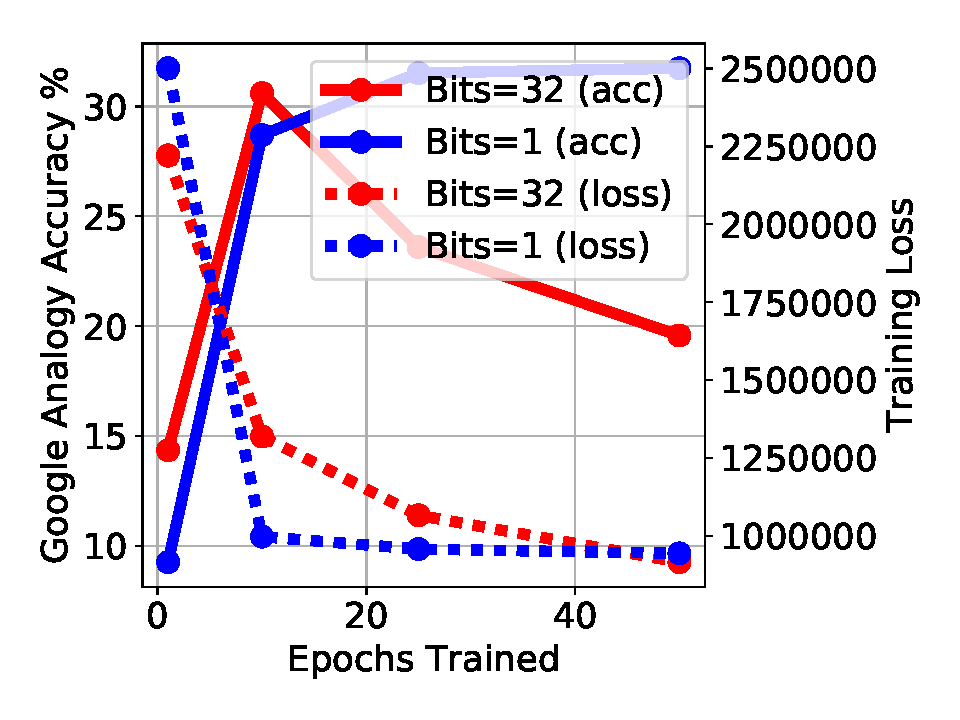
\includegraphics[width=6cm]{images/Wiki8AccuracyVsEpochsTrainedDimension=400.pdf}}}%
    \qquad
    \subfloat[Training loss and accuracy vs dimension (epochs trained = 10)]{{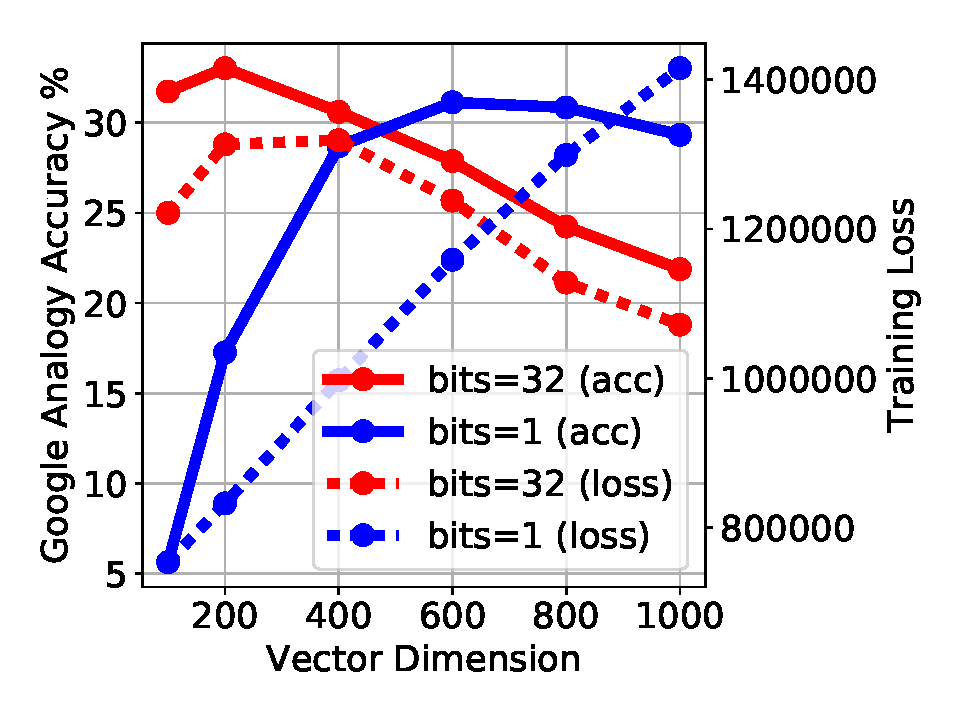
\includegraphics[width=6cm]{images/Wiki8AccuracyVsDimensionEpochsTrained=10.pdf} }}%
    \caption{Overfitting in Word2Vec; regularization in Word2bits}%
    \label{fig:overfitting}
\end{figure}

\subsection{Word2Bits Visualization}


\section{Discussion and Future Work}

\subsubsection*{Acknowledgments}

\subsubsection*{References}

\small{ [1] Alexander, J.A. \& Mozer, M.C. (1995) Template-based
  algorithms for connectionist rule extraction. In G. Tesauro,
  D. S. Touretzky and T.K. Leen (eds.), {\it Advances in Neural
    Information Processing Systems 7}, pp. 609-616. Cambridge, MA: MIT
  Press.

- COMPRESSING WORD EMBEDDINGS VIA DEEP COMPOSITIONAL CODE LEARNING
- FASTTEXT.ZIP: COMPRESSING TEXT CLASSIFICATION MODELS
- FASTTEXT (Bag of Tricks for Efficient Text Classification)
- Intrinsic Evaluation of Word Vectors Fails to Predict Extrinsic Performance
- Improving Distributional Similarity with Lessons Learned from Word Embeddings
- Optimal brain damage
- Second order derivatives for network pruning: Optimal brain surgeon
- Learning both weights and connections for efficient neural networks
- Distributed Representations of Words and Phrases and their Compositionality
- Efficient Estimation of Word Representations in Vector Space
- Binarized Neural Networks
- Hinton, Geoffrey. Neural networks for machine learning. Coursera, video lectures, 2012.
- GloVe: Global Vectors for Word Representation
- Learned in Translation: Contextualized Word Vectors
- HALP
- Towards Lower Bounds on Number of Dimensions for Word Embeddings
- Evaluation methods for unsupervised word embeddings
- SQuAD
- DrQA
- WordSim353 Finkelstein
- WordSim Similarity, WordSim Relatedness (Zesch et al., 2008; Agirre et al., 2009
- Bruni et al.s (2012) MEN
- Radinsky et al.s (2011) Mechanical Turk
- Luong et al.s (2013) Rare Words dataset
- Hill et al.s (2014) SimLex-999
- Low precision arithmetic for deep learning.
- Predicting parameters in deep learning
- Compressing neural networks with the hashing trick
- Compression of Neural Machine Translation Models via Pruning
- Reading Wikipedia to Answer Open-Domain Questions
\end{document}
